\documentclass{article}
\usepackage[utf8]{inputenc}
\usepackage{amsmath}
\usepackage{natbib}
\usepackage{graphicx}
\usepackage[utf8]{inputenc}
\usepackage[english,russian]{babel}
\usepackage{cmap}
\usepackage{float}
\usepackage{amsmath,amssymb}
\usepackage{pythonhighlight}

\begin{document}
	
\section{Метод моментов}
\subsection{Равномерное распределение}
Методом моментов оценить параметры равномерного распределения. 
\subsubsection{Решение}
Пусть случайная величина $X$ распределена равномерно на отрезке $[a, b]$:
\[X \sim R[a, b]\]
Тогда посчитаем математическое ожидание и дисперсию $X$:
\[\mathbb{E}X = \int_{-\infty}^{+\infty}xdF_X(x) = \int_{-\infty}^{+\infty}xf_X(x)dx = \int_{a}^{b}x*\frac{1}{b-a}dx = \frac{b+a}{2}\]
\[\mathbb{E}X^2 = \int_{-\infty}^{+\infty}x^2dF_X(x) = \int_{-\infty}^{+\infty}x^2f_X(x)dx = \int_{a}^{b}x^2*\frac{1}{b-a}dx = \frac{b^2+ab+a^2}{3}\]
\[\mathbb{D}X = \mathbb{E}X^2 - (\mathbb{E}X)^2 = \frac{4b^2+4ab+4a^2 - 3b^2 - 6ab - 3b^2}{12} = \frac{(b-a)^2}{12}\]
Используя моменты, являющиеся несмещенными и СК-состоятельными оценками $\mathbb{E}X$ и $\mathbb{D}X$, для выборки $\mathbb{X}$ длины n:
\[\overline{X} = \frac{1}{n}\sum_{i = 1}^{n}X_i;\]
\[\overline{\mu_{n,2}} = \frac{1}{n-1}\sum_{i = 1}^{n}(X_i - \overline{X})^2\]

Получаем систему:
\begin{equation*}
\begin{cases}
	\mathbb{E}X = \overline{X} &,\\
	\mathbb{D}X = \overline{\mu_{n, 2}}
\end{cases}
\end{equation*}

После подстановки теоретических значений приходим к следующему:
\begin{equation*}
	\begin{cases}
		a = \overline{X} - \sqrt{3\overline{\mu_{n, 2}}} &,\\
		b = \overline{X} + \sqrt{3\overline{\mu_{n, 2}}}
	\end{cases}
\end{equation*}

Смоделируем выборку длины 100 и 100000 с фикисрованными параметрами a и b, затем используем метод моментов и сравним полученные значения с теоретическими.

Запрограммируем метод моментов на языке Python:
\begin{python}
def R_moments(mas):
	x_mean = mas.sum()/len(mas)
	disp_mas = (mas - x_mean)**2
	x_disp = disp_mas.sum()/(len(disp_mas)-1)
	a = x_mean - np.sqrt(3*x_disp)
	b = x_mean + np.sqrt(3*x_disp)
	print('R[' + str(a)+', '+str(b)+']')
\end{python}

Выберем значения a и b равными 2 и 5 $X \sim R[2, 5]$, соответственно.
Для генерации выборки используем модуль numpy:
\begin{python}
import numpy as np
\end{python}

Выборка длины 100:
\begin{python}
mas = np.random.uniform(low = 2.0, high = 5.0, size = (100))
R_moments(mas)
\end{python}
Результат работы:
R[1.9324522786552465, 5.143832231571253]

Выборка длины 100000:
\begin{python}
mas = np.random.uniform(low = 2.0, high = 5.0, size = (100000))
R_moments(mas)
\end{python}
Результат работы:
R[2.000739652113247, 5.0031579304426455]

\subsection{Экспоненциальное и сдвинутое экспоненциальное распределение}
Методом моментов оценить параметры экспоненциального и сдвинутого экспоненциального распределений. 
\subsubsection{Решение}
Рассмотрим случайную величину, распределенную экпоненциально с параметром $\lambda$: $X \sim Exp(\lambda)$

Посчитаем $\mathbb{E}X$ и $\mathbb{D}X$:
\[\mathbb{E}X = \int_{-\infty}^{+\infty}xf_X(x)dx = 0 + \int_{0}^{+\infty}x\lambda e^{-\lambda x}dx = \int_{0}^{+\infty}-xde^{-\lambda x} = \]
\[=\left.-xe^{-\lambda x}\right|_{0}^{+\infty} + \int_{0}^{+\infty}e^{-\lambda x}dx = \left.-\frac{1}{\lambda}e^{-\lambda x}\right|_{0}^{+\infty} = \frac{1}{\lambda}\]
\[\mathbb{E}X^2 = \int_{-\infty}^{+\infty}x^2f_X(x)dx = 0 + \int_{0}^{+\infty}x^2\lambda e^{-\lambda x}dx = \int_{0}^{+\infty}-x^2de^{-\lambda x} =\]
\[=\left.-x^2e^{-\lambda x}\right|_{0}^{+\infty} + \int_{0}^{+\infty}e^{-\lambda x}dx^2 = 2\times\int_{0}^{+\infty}xe^{-\lambda x}dx = \frac{2}{\lambda}\mathbb{E}X = \frac{2}{\lambda^2}\]
\[\mathbb{D}X = \mathbb{E}X^2 - (\mathbb{E}X)^2 = \frac{1}{\lambda^2}\]

Используя несмещенную и СК-состоятельную оценку $\mathbb{E}X$, получим:
\[\mathbb{E}X = \overline{X} => \frac{1}{\lambda}=\overline{X} => \lambda = \frac{1}{\overline{X}}\]

Запрограммируем метод моментов для экспоненциального распределения на языке Python:
\begin{python}
def Exp_moments(mas):
	x_mean = mas.sum()/len(mas)
	l = 1/x_mean
	print('Exp[' + str(l) + ']')
\end{python}

Для примера рассмотрим распределение с параметром 5: $X \sim Exp(5)$.

Используем модуль numpy для генерации выборок. Выборка длины 100(
$scale = beta = \frac{1}{\lambda}$, $beta$ - аргумент метода exponential):
\begin{python}
exp = np.random.exponential(scale = 1/5, size = (100))
Exp_moments(exp)
\end{python}
Результат работы:
Exp[4.452551487118613]

Выборка длины 100000:
\begin{python}
exp = np.random.exponential(scale = 1/5, size = (100000))
Exp_moments(exp)
\end{python}
Результат работы:
Exp[4.974561792226967]

Теперь смоделируем сдвинутое экспоненциальное распределение.

Так как в модуле numpy нет соответствующего метода, найдем обратную функцию распределения и используем генератор для получения нужной выборки:

\[X \sim Exp(\lambda, x_0)\]
\begin{equation*}
	F_X(x) = 
	\begin{cases}
		1 - e^{-\lambda(x-x_0)} &, x >= x_0,\\
		0 &, x < x_0
	\end{cases}
\end{equation*}


\[Y = 1 - e^{-\lambda(x-x_0)} => x = x_0 + \frac{1}{\lambda} \times \ln{\left(\frac{1}{1-Y}\right)}\]
Тогда 
\[X = x_0 + \frac{1}{\lambda} \times \ln{\left(\frac{1}{1-R[0, 1]}\right)} \sim Exp(\lambda, x_0)\]

Посчитаем $\mathbb{E}X$ и $\mathbb{D}X$:
\[\mathbb{E}X = 0+\int_{x_0}^{+\infty}xf_X(x)dx = \int_{x_0}^{+\infty}(x-x_0)\lambda e^{-\lambda(x-x_0)}d(x-x_0) +\]
\[+ \int_{x_0}^{+\infty}x_0\lambda e^{-\lambda(x-x_0)}dx = x_0 + \mathbb{E}Exp(\lambda, 0) = x_0 + \frac{1}{\lambda}\]
\[\mathbb{D}X = \mathbb{D}[X- x_0 + x_0] = \mathbb{D}[X-x_0] = \mathbb{D}[Exp(\lambda, 0)] = \frac{1}{\lambda^2}\]

Для примера рассмотрим сдвинутое экспоненциальное распределение с параметрами $\lambda = 5; x_0 = 3$.
Проверим смоделированную величину, изобразим эмперическую функцию распределения и теоретическую на одном графике для дувух выборок:

\begin{figure}[H]
	\center{
		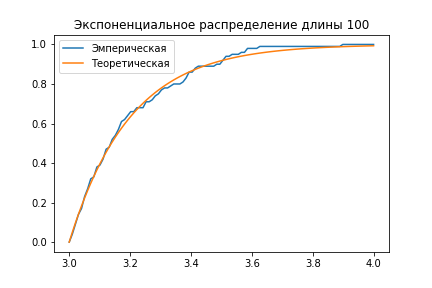
\includegraphics[scale=0.39]{./Task_2_2/Exp_100.png}
		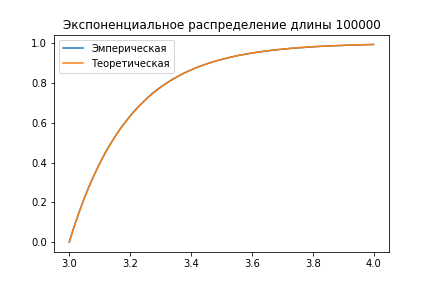
\includegraphics[scale=0.39]{./Task_2_2/Exp_100000.png}
	}
	\caption{Сдвинутое экспоненциальное распределение Exp(5, 3)}
	\label{fig:image}
\end{figure}

Используем несмещенные и СК-состоятельные оценки $\mathbb{E}X$ и $\mathbb{D}X$:
\begin{equation*}
	\begin{cases}
		\mathbb{E}X = \overline{X} &,\\
		\mathbb{D}X = \overline{\mu_{n, 2}}
	\end{cases}
\end{equation*}

После подстановки получим:
\begin{equation*}
	\begin{cases}
		x_0 + \frac{1}{\lambda} = \overline{X} &,\\
		\frac{1}{\lambda^2} = \overline{\mu_{n, 2}}
	\end{cases}
\end{equation*}
Тогда:
\begin{equation*}
	\begin{cases}
		x_0 = \overline{X} - \frac{1}{\lambda} &,\\
		\lambda = \sqrt{\frac{1}{\overline{\mu_{n, 2}}}}
	\end{cases}
\end{equation*}
Или же:
\begin{equation*}
	\begin{cases}
		x_0 = \overline{X} - \sqrt{\overline{\mu_{n, 2}}} &,\\
		\lambda = \sqrt{\frac{1}{\overline{\mu_{n, 2}}}}
	\end{cases}
\end{equation*}

Запрограммируем описанный метод на языке Python:
\begin{python}
def Exp_moments1(mas):
	x_mean = mas.sum()/len(mas)
	disp_mas = (mas - x_mean)**2
	x_disp = disp_mas.sum()/(len(disp_mas)-1)

	l = 1/np.sqrt(x_disp)
	x_0 = x_mean - 1/l
	print('Exp[' + str(l) + ', ' + str(x_0) + ']')
\end{python}

Выборка длины 100:
\begin{python}
exp1 = exp(5, 3)
Exp_moments1(exp1)
\end{python}

Результат работы:
Exp[5.625025698971059, 3.0159937655655447]


Выборка длины 100000:
\begin{python}
exp2 = exp(5, 3, size = 100000)
Exp_moments1(exp2)
\end{python}

Результат работы:
Exp[4.9870433076067355, 2.9991436233274964]

\subsection{Распределение Коши}
Плотность распределения Коши имеет вид
\[f_X(x) = \frac{1}{\pi}\frac{\gamma}{(x-x_0)^2+\gamma^2}\]
а функция распределения – 
\[F_X(x) = \frac{1}{\pi}\arctan{\left(\frac{x-x_0}{\gamma}\right)} + \frac{1}{2}\]
Подобрать функции $g_1(x)$ и $g_2(x)$, так, чтобы с помощью соответствующих моментов методом моментов можно было оценить параметры сдвига и масштаба распределения Коши. 
\subsubsection{Решение}
Распределение Коши не имеет моментов, поэтому оценивать величину сдвига и масштаба будем через эмперическую функцию распределения и гистограмму.

Плотность распределения Коши:
\[f_X(x) = \frac{\gamma}{\pi*\left(\gamma^2+(x-x_0)^2\right)}\]

Функция распределения:
\[F_X(x) = \frac{1}{\pi}\arctan{\left(\frac{x-x_0}{\gamma}\right)} + \frac{1}{2}\]

Так как в модуле numpy нет распределения Коши с произвольными параметрами, смоделируем искомую величину через обратную функцию, как это было в ДЗ №1, но в произвольном случае, то есть не только в случае $C(0, 1)$:
\[F_X^{-1}(x) = x_0 + \gamma\tan{\left[\pi\left(x - \frac{1}{2}\right)\right]}\]

Заменим x на $R[0, 1]$, получим искомую.

Запрограммируем данный способ на языке Python:
\begin{python}
def C_t(size = 100, x_0 = x_0_6, gamma = gamma):
	return x_0 + gamma * np.tan(np.pi * (np.random.uniform(size = size) - 1/2))
\end{python}

Чтобы применить метод моментов, рассмотрим смещение распределения $x = x_0$ и заметим, что это смещение является медианой:
\[F_X(x_0) = \frac{1}{2}; f_X(x_0) =  \frac{\gamma}{\pi*\left(\gamma^2+0\right)} = \frac{1}{\pi\gamma}\]

Тогда получаем, что $x_0$ можно выбирать как медиану выборки, а параметр $\gamma$ определяется из следующих рассуждений(k - число разрядов гистограммы):
\[h(x_0) \underset{k \to +\infty}{\longrightarrow} f_X(x_0) = \frac{1}{\pi\gamma} => \gamma = \frac{1}{\pi h(x_0)}\]

Для ускорения вычислений приходится уменьшить число разрядов гистограммы, поэтому ниже приведены примеры для выборки длины 100 и числа разрядов 150, а также для выборки длины 10000 и числа разрядов 1000.

Для примера рассмотрено распределение с параметрами $\gamma = 1.5; x_0 = 5$, то есть x\_0\_6 = 5 в коде выше, а gamma = 1.5.
Для наглядности добавлены графики плотности вероятности и гистограмма двух выборок.

Запрограммируем формулу вычисления гистограммы(x - аргумент функции гистограммы, n\_c - число разрядов,
result - массив, хранящий число элементов выборки в каждом разряде, mas - массив точек, ограничивающий каждый раязряд($a_i$ в разбиении числовой прямой)):

\begin{python}
def hc(x, n_c, result, mas, n):
	ans = 0
	for j in range(n_c):
		if x <= mas[j+1] and x > mas[j]:
			ans += result[j] / (mas[j+1] - mas[j])
	ans /= n
	return ans
\end{python}

Запрограммируем метод моментов и построение гистограммы для распределения Коши:
\newpage
\begin{python}
def Cauch_moments(inp):
	median = np.sort(inp)[int(len(inp)/2) - 1]

	start = int(inp.min()) - 1
	stop = int(inp.max()) + 1
	x = np.linspace(start= start, stop=stop, num=len(inp))

	if(len(inp) <= 100):
		n_c = 150
	else:
		n_c = 1000
	hist_len = (x.max() - x.min())/(n_c)
	mas = np.zeros((n_c+1))

	for i in range(n_c):
		mas[i] = x.min() + hist_len*i
	mas[n_c] = x.max()

	result = np.zeros((n_c))
	c = inp
	for i in range(len(c)):
		for j in range(n_c):
			if c[i] <= mas[j+1] and c[i] > mas[j]:
				result[j] += 1

	fx = lambda x: 1/np.pi * 1.5/((x - 5)**2 + 2.25)
	plt.plot(x, h1(x, n_c, result, mas))
	plt.plot(x, fx(x))
	sum = 0;
	for i in range(len(inp)):
		sum += hc(inp[i], n_c, result, mas, len(c))
	sum /= len(inp)
	gamma = 1/(np.pi*hc(median, n_c, result, mas, len(c)))
	print("C(" + str(median) + ", " + str(gamma) + ')')
	plt.legend(["Bar graph", "Distribution density"])
	plt.title("Cauchy distribution of length " + str(len(inp)))
	plt.savefig("./Task_2_3/Cauch_"+str(len(inp))+".png")	
\end{python}

Смоделируем выборку длины 100:
\begin{python}
cau1 = C_t()
Cauch_moments(cau1)
\end{python}
Результат работы:
C(4.750004117181387, 1.3606187291777851)
\begin{figure}[H]
	\center{
		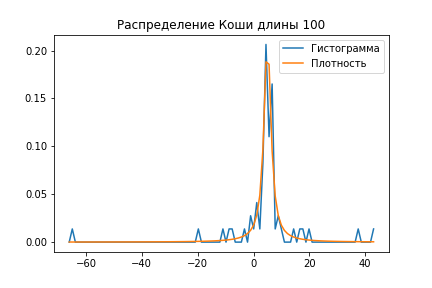
\includegraphics[scale=0.5]{./Task_2_3/Cauch_100.png}
	}
	\caption{Выборка длины 100}
	\label{fig:image}
\end{figure}

Смоделируем выборку длины 10000:
\begin{python}
cau2 = C_t(size = 10000)
Cauch_moments(cau2)
\end{python}
Результат работы:
C(4.98376276044115, 2.643928460393461)
\begin{figure}[H]
	\center{
		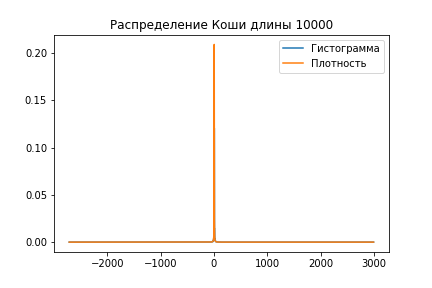
\includegraphics[scale=0.5]{./Task_2_3/Cauch_10000.png}
	}
	\caption{Выборка длины 100}
	\label{fig:image}
\end{figure}
\end{document}